\documentclass[letterpaper,11pt]{article}

\usepackage[hidelinks]{hyperref}
\usepackage[empty]{fullpage}
\usepackage{parskip}
\usepackage{graphicx}
\usepackage{float}
\usepackage{booktabs}
\usepackage{tabularx}
\usepackage[table]{xcolor}
\usepackage{geometry}
\usepackage{amsmath}
\usepackage{enumitem}
\usepackage{cleveref}
\usepackage{calc}

% Ensure that the generated pdf is machine readable/ATS parsable
\pdfgentounicode=1


\begin{document}

\begin{center}
    \textbf{\Huge Societal Problem Definition}
\end{center}

\subsection*{Article}

\textbf{Author:} Megan Cerullo, CBS News \\
\textbf{Updated on:} May 22, 2026 / 11:17 PM EDT \\
\textbf{Link:} \href{https://www.cbsnews.com/news/ai-layoffs-hiring-entry-level-workers/}{https://www.cbsnews.com/news/ai-layoffs-hiring-entry-level-workers/} \\
\textbf{Editor:} Aimee Picchi \\
\textbf{Additional contributors:} Mary Cunningham

% \textbf{AI job cuts are rising, but experts say layoffs are only part of the story}

AI-related layoff announcements are mounting, fueling the sense that the technology is already replacing a significant number of U.S. workers as companies invest heavily in automation. But AI's broader impact on workers may be quieter: weaker hiring, especially for junior and entry-level roles.

Enterprise software maker Intuit this week cut 17\% of its staff, or 3,000 people, saying it would shift its focus to AI, while Meta began laying off 8,000 workers on Wednesday as it shifts investment toward AI. Last week, Cisco also announced thousands of job cuts, with CEO Chuck Robbins saying in a blog post that it was reducing headcount in part to invest in "employees' use of AI across the company."

Andrew Tran, 40, a Meta product designer who was among those losing their job this week, told CBS News he plans to look for a new job at a company that he believes is using AI "intentionally," rather than chiefly to replace workers.

Tran doesn't believe his role at Meta was directly replaced by AI, but said it's clear corporations are leaning into the tech.

"In general, companies should have an obligation to retrain their workforces instead of throwing them to the curb," he told CBS News, while clarifying that his views are aimed at the corporate sector as a whole and not specifically at Meta.

Meta didn't immediately reply to a request for comment.
Thousands of job cuts

Companies have announced nearly 50,000 job cuts this year linked to AI, according to research from outplacement firm Challenger, Gray \& Christmas. Those layoffs account for roughly 17\% of the roughly 300,000 total job cuts announced so far in 2026, the firm's figures show.

The layoffs come as some analysts warn AI could eventually reshape the labor market on a much larger scale. Boston Consulting Group has projected that up to 15\% of U.S. jobs could be eliminated over the next five years.

Economists say that most of the recent AI-related layoffs are limited to the high-tech sector, while noting that companies may not always adopt such tools as a direct substitute for workers.

"We are seeing a lot of layoff announcements that are supposedly related to greater use of AI," EY-Parthenon chief economist Greg Daco told CBS News. "They are aimed at cutting down on labor expenses, while AI investment is growing very rapidly, but I'm not entirely sure this is a replacement situation where talent is being replaced by technology."

Some economists say AI's impact on the labor market may be emerging less through mass layoffs and more through weaker hiring. Some companies are delaying recruitment while they evaluate how AI changes their staffing needs, potentially making it tougher for younger and entry-level workers to find jobs.

In other words, these businesses may not be laying off workers, but they're also not creating new jobs.
Junior workers squeezed

Lackluster hiring can draw less attention than layoffs because companies rarely announce such decisions. Research from Goldman Sachs shows that in the past year, AI reduced monthly payroll growth by roughly 16,000 jobs, raising the unemployment rate by 0.1 percentage point.

"AI seems to be impacting labor finally, but it's actually not so much through increased layoffs. The main channel tends to be reduced hiring, especially reduced hiring of junior workers," Daniel Keum, associate professor of management at Columbia Business School, told CBS News.

Younger workers may face particular challenges because entry-level roles are easier to automate than senior positions, experts said.

"The major sort of impact of AI will come from reduced hiring of juniors," Keum said, noting that "seniors are a lot more difficult to replace."

AI may also reshape job requirements, creating new roles that do not necessarily align with the skills of workers displaced by automation.

"The people who get laid off don't necessarily get the next set of jobs, because the roles are different," said Ken Matos, an organizational psychologist and director of insights at hiring platform HiBob.

Still, he expects hiring to rebound after companies complete major AI investments.

"Right now, companies are moving labor dollars into tech investment," Matos said. "Hopefully, that moves back into labor dollars once the technology is set up."
Positive spin

Corporations are also grappling with a host of other pressures, such as geopolitical tensions, fluctuating U.S. tariff policy and other sources of economic uncertainty, which could be driving layoffs and crimping hiring.

But framing workforce cuts as part of an AI strategy may send a more positive signal to investors than citing weaker demand or rising costs, Daco said.

"When you announce layoffs in general, it's not seen as a good thing from markets' and investors' perspectives," Daco said. "But when you say you're proceeding with layoffs because of AI, it's positive from a communications standpoint."

Attributing job cuts to AI can help companies "frame a complex picture into a simple message that is easily understood," said Clarence Lee, a tech entrepreneur and professor at the Cornell SC Johnson College of Business.

Only about 10\% of firms currently use AI to produce goods and services, and only a subset are replacing workers with the technology, according to Daco.

"There is some job displacement, but we are not seeing massive job dislocation as a result of AI at this stage," he said.

Dan Freedman, a Google software engineer and member of the Alphabet Workers Union, sees a link between the recent jump in layoffs and the push to embrace AI, while noting that he doesn't believe the tech is replacing workers "one for one."

"AI is just the latest fear about our jobs that we have to work through now," he told CBS News.
What should workers do?

Experts say workers who combine AI skills with adaptability may be best positioned as the labor market evolves.

"AI is a dynamic beast, so we are now looking for the ability to accept risk, people who are motivated by continuous learning, who are engaged by the transformation," Matos said. "It's a personality trait as much as it's a skill-set."

Lee said workers should focus on understanding what AI can do while identifying skills that remain uniquely human.

"That's where the magic unlocks," he said.

\begin{figure}[H]
    \centering
    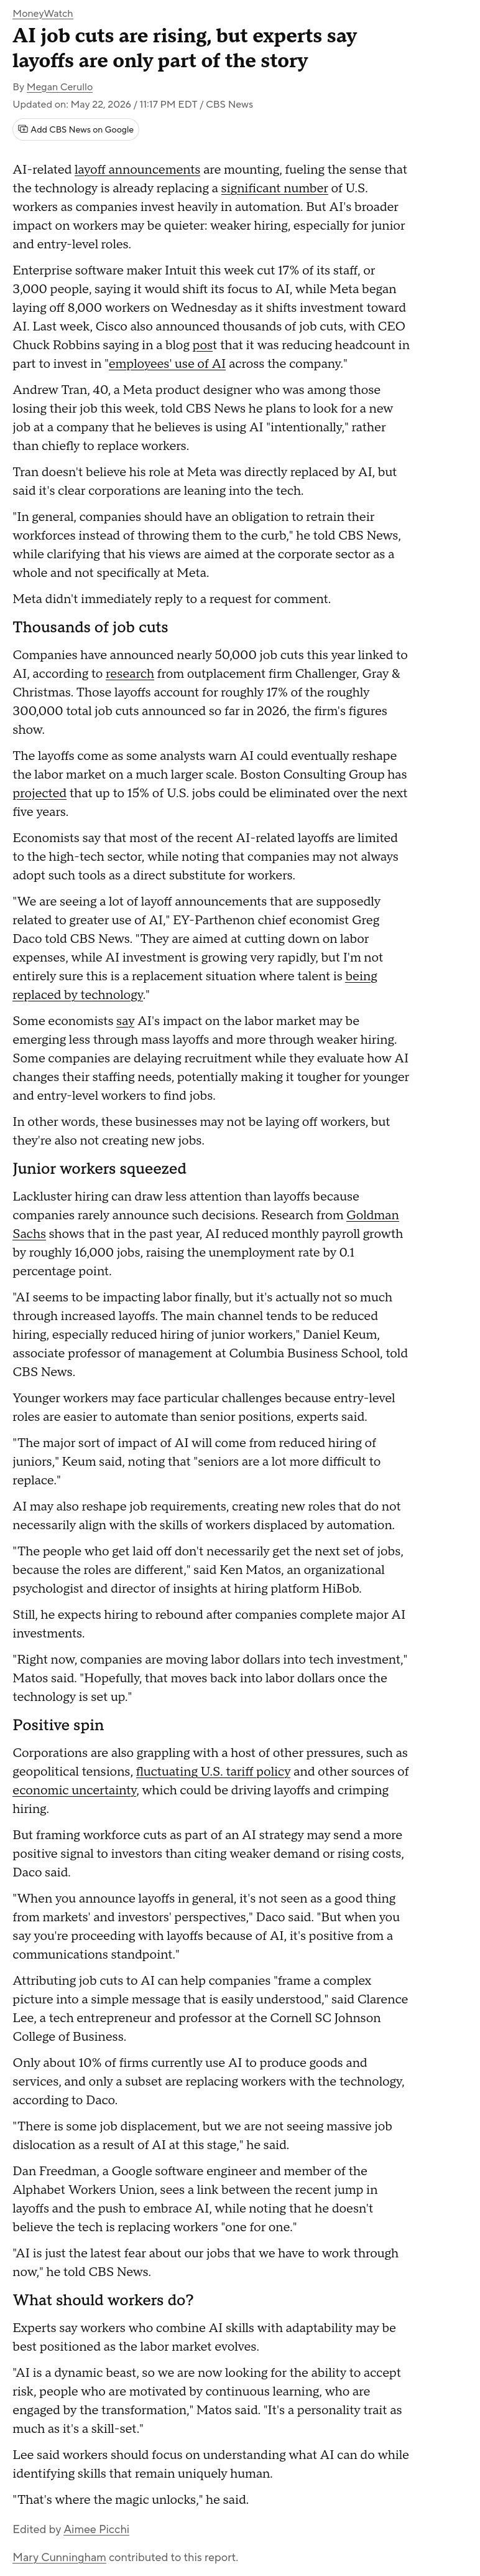
\includegraphics[width=\textwidth,height=\textheight-134pt,keepaspectratio=true]{article.png}
    % \caption{}
    % \label{fig:...}
\end{figure}


\subsection*{The Challenge}
The societal problem described in this article is about how AI
automatization and usage affects the job market. It suggests that AI
has made it more difficult for junior workers to find a new workplace
while also reducing available job offers and potentially being cause
for layoffs.

\begin{enumerate}[label=(\alph*)]
    \item {
          We are interested in this particular topic, because AI is a big part of
          this Bachelor's degree, and we found it interesting to discuss how it
          can affect our future employment.
          }
    \item {
          The main stakeholders here are the working population and those that are soon to
          (attempt to) join the workfore, especially newly graduated students who would aim
          for the junior positions which this article suggests are in low supply. One other
          group that feels the effect of this issue are those not laid off, as they are left
          to deal with having lost their coworkers and potentially fearing being the next
          ones to go.
          }
\end{enumerate}


\subsection*{Papers}

\textbf{Reference:} \cite{employment2024rizun} \\
\textbf{Subtype of article:} Original peer-reviewed conference paper (empirical study).

This paper explains how AI and rapid digitalization are shifting requirements
for young graduates transitioning from higher education to the labor market.
The authors illustrate that entry-level job security is challenged as AI
increasingly takes over baseline cognitive tasks that traditionally served
as learning grounds for junior employees. Crucially, the study highlights
an emerging skills gap, showing that academic curricula must pivot toward
non-automatable skills alongside AI literacy.

---

\textbf{Reference:} \cite{stealingjobs2024eric} \\
\textbf{Subtype of article:} Original research article

This article investigates job displacement related to artificial intelligence.
The study examines whether workers have actually experienced a job loss related to a rise of AI
and which types of workers are more vulnerable to displacement. The research was based
on a survey of 1000 employed adults in the United States. Participants were asked
about their experience with AI in the workplace and whether they had been replaced by it
before. The results showed that 12.6\% of respondents that they had previously lost their
jobs because of AI. The result also showed that around 20\% of respondents working in
non-routine cognitive occupations reported AI-related job displacement,
compared with 8\% working in other occupations. Which show that white-collar jobs
may be more vulnerable to AI job displacement.

---

\textbf{Reference:} \cite{abraham_solaja_artificial_2025} \\
\textbf{Subtype of article:} Original research article

The article explores and (attempts to) define the psychological archetypes of those
employees who managed to "survive" the layoffs, but are now left to deal with
the consequences, in this case, the psychological aspects of being a "survivor".
There are four main types/groups of people that are being distinguished: Empowered
Adapters, Hopeful Dependents, Quiet Quitters, and Fear-Driven Adapters. The article
does empahsize that people don't usually neatly fit in those categories, however, they
can be used as a tool to help deal with certain issues. One main issue is the fear of
"being the next one" and such fears or job insecurity lead to increase psychological
stress, which naturally has overall negative consequences. Though there are also people
that instead turn it around and use these changes to improve themselves. Overall, the
article puts forth several propositions which might be beneficial for both employees
and employers to deal with the situation caused by these AI-related layoffs, as well as,
in some capacity encourage employees to realize their ability to improve their outcomes
in such situations.


\bibliographystyle{apalike}
\bibliography{references}

\end{document}
